\clearpage
\section{原理}
\subsection{追記:半導体(semiconductor)}
室温付近で金属と絶縁体(不導体)の中間の電気抵抗値を示すもの.
金属と異なり,温度が増加すると共に電気抵抗は減少する.
これらは,4価のシリコン(Si)がよく用いられる真性半導体(intrinsic semiconductor),不純物半導体(extrinsic semiconductor)に大きく分類される.
また,不純物半導体は半導体に微量の不純物を混入させたものをいい,
この不純物により電気抵抗が大きく変化する.
半導体のエネルギーバンドを\wfig{semi-band}に示す.

\begin{figure}[h]
	\centering
	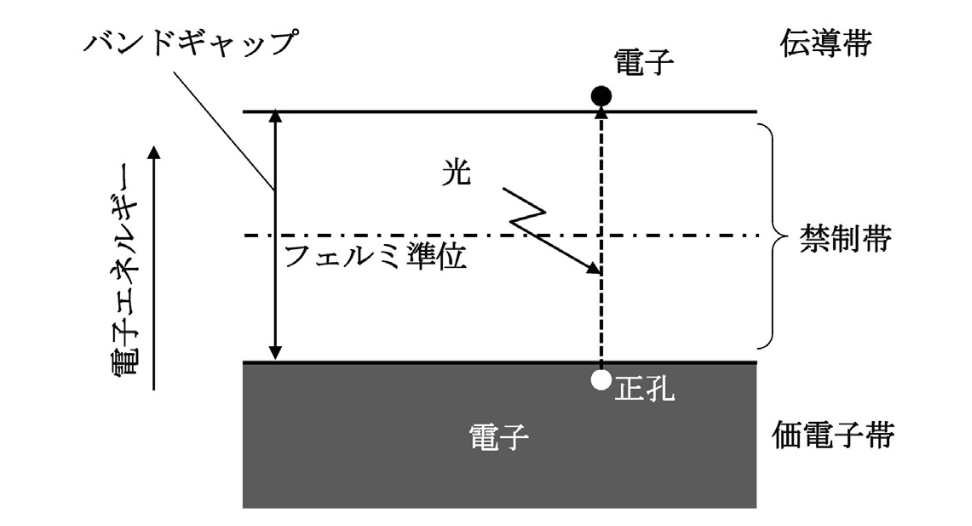
\includegraphics[scale=0.8]{./fig/semi-band.png}
	\caption{半導体のエネルギーバンド\cite{sdfnvd}}
	\label{fig:semi-band}
\end{figure}

\subsection{追記:p型半導体(p-type semiconductor)}
不純物半導体の一種で,ホウ素やガリウムのような3価の元素(acceptor, アクセプタ)を用いたもの.
多数キャリアは正孔である.

\subsection{追記:n型半導体(n-type semiconductor)}
不純物半導体の一種で,不純物としてリン(P)やヒ素(As)のような5価の元素(donor, ドナー)を用いたもの.
多数キャリアは電子である.

\subsection{変更:ダイオード(diode)}
\wfig{fig1}のように,p型半導体とn型半導体を接合し,端子を付けたものをダイオードと呼ぶ.
ダイオード内部において,正孔はp型半導体内では多数キャリア,n型半導体内では少数キャリアであるから,より密度の大きいp型領域からn型領域へ流れ込む.
この現象を拡散(diffusion)と呼ぶ.
また,n領域へ拡散した正孔はn領域内の電子と結合し,双方とも消滅する.
したがって,n領域では正に帯電したドナーイオンが,p領域では負に帯電したアクセプタイオンのみが残り,平衡状態となる.
この結果,pn接合近傍にはキャリアの存在しない空乏層(depletion layer)が形成される.
空乏層では,電位分布によりp領域側からn領域側へ電位差が発生し,これを拡散電位と呼ぶ.

\begin{figure}[!h]
 \centering
 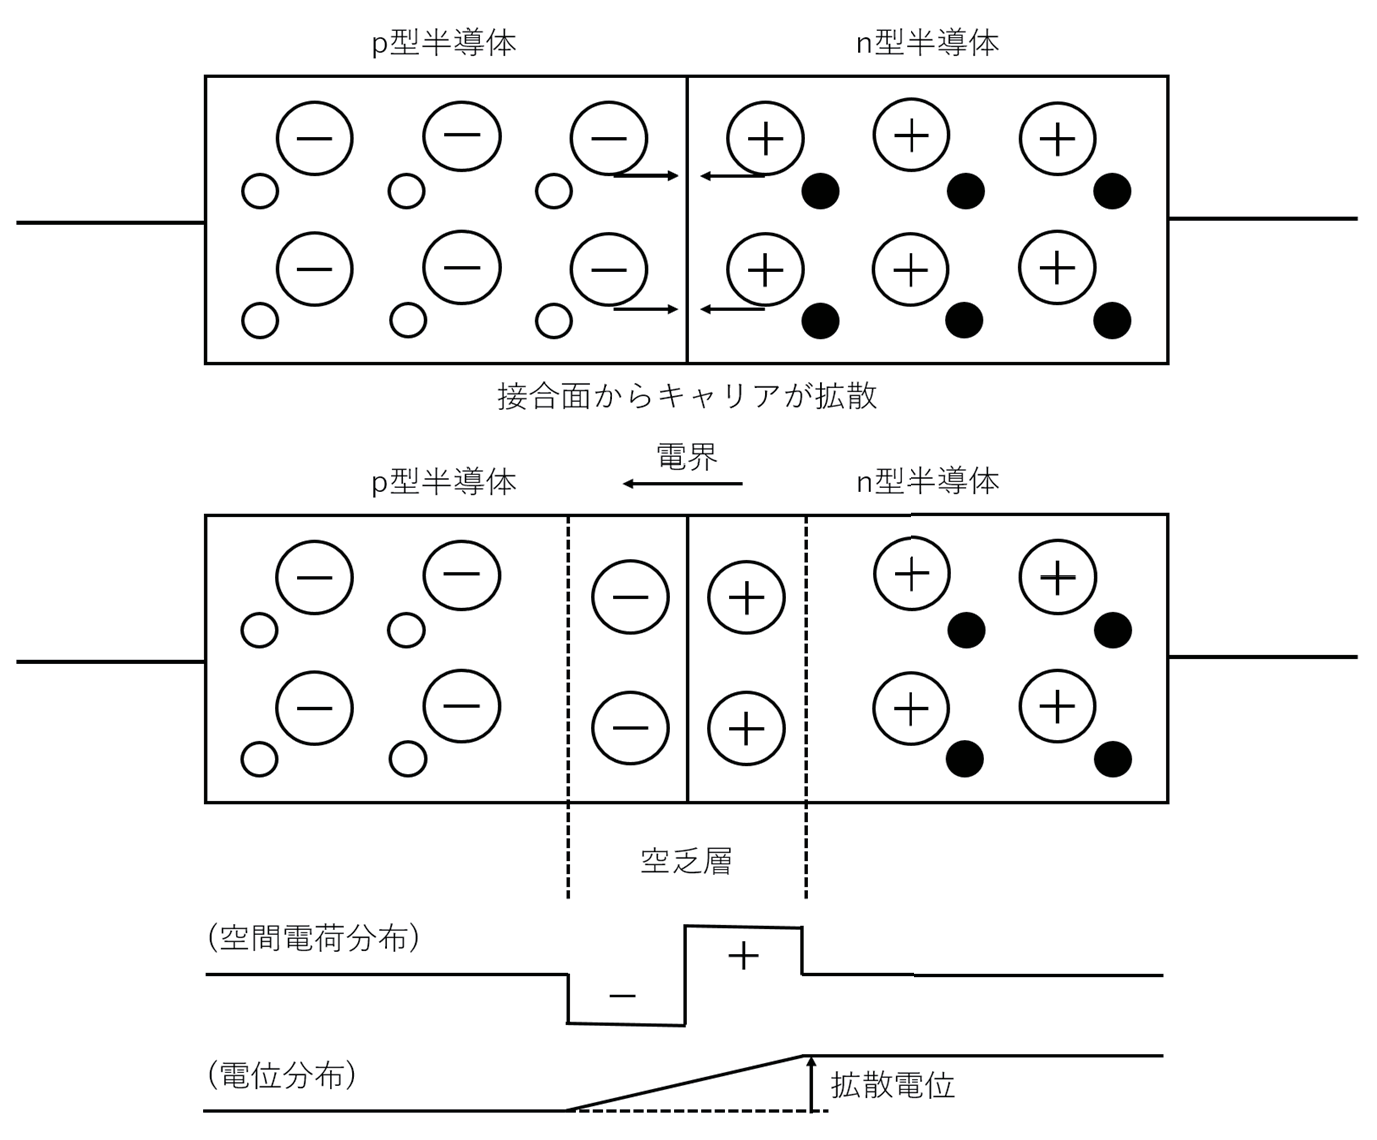
\includegraphics[width=8.2cm]{./fig/fig1.eps}
 \caption{pn接合と空乏層}
 \label{fig:fig1}
\end{figure}%

\wfig{fig2}のようにp型半導体に正,n型半導体に負の電圧を加えると,p領域とn領域の電位差は拡散電圧+印加電圧となり,電圧差が減少するため拡散電位により阻止されていたキャリアの拡散が起こる.
このとき,ダイオードに印加した電圧,流れた電流を,それぞれ順方向電圧,順方向電流という.
逆に,n型半導体に正,p型半導体に負の電圧を加えると,p領域とn領域の電圧差が大きくなるため電流は殆ど流れなくなる.
このとき,ダイオードに加えた電圧,流れた電流を,それぞれ逆方向電圧,逆方向電流という.
また,この電圧印加方法を逆バイアス(reverse bias)という.

\begin{figure}[!t]
 \centering
 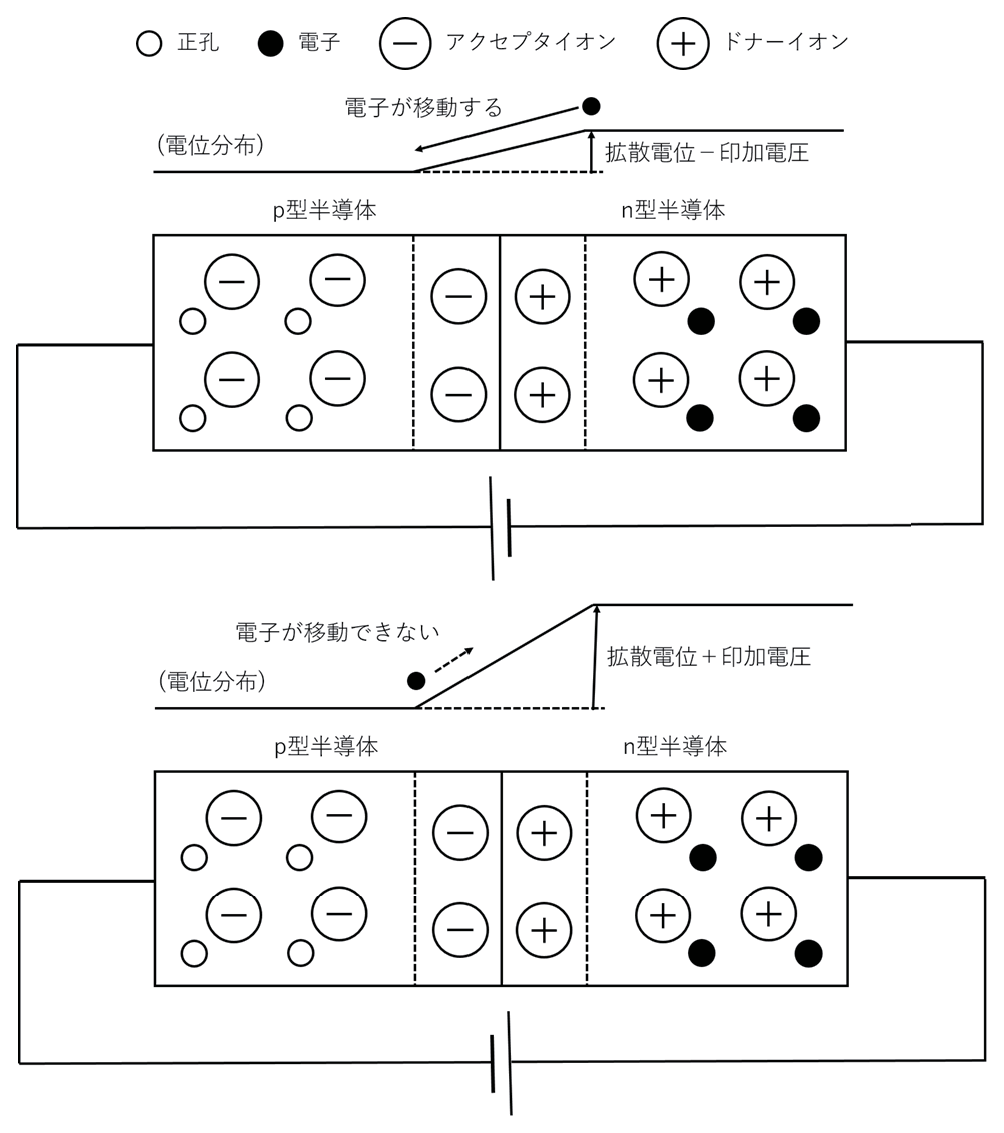
\includegraphics[height=8.0cm]{./fig/fig2.eps}
 \caption{ダイオードの動作原理}
 \label{fig:fig2}
\end{figure}%

\subsection{変更:ツェナーダイオード(Zener diode)}
ツェナーダイオードは定電圧ダイオードとも呼ばれ,加わる電圧がある一定の値(ツェナー電圧)を上回ると,急激に電流が流れるようになる素子である.
このとき流れる電流をツェナー電流(Zener current)と呼ぶ.
入力電圧の増加に伴いツェナー電流が増加するため,出力電圧は一定に保たれる.
すなわち,ツェナーダイオードは端子間電圧がツェナー電圧以上ならON,ツェナー電圧以下ならOFFといったようにスイッチと似たような動作をして,ほぼ一定の電圧を維持する素子である.

\subsection{追記:負荷線(load line)\cite{1130282271098}\cite{1130000795906158592}}
印加する電圧を直流成分のみであるとして立式した,コレクタ直流電流の式($I_{C}=$)のことである.
$I_{C}=0$とすることによりコレクタ電圧$V_{CC}$が,$V_{CC}=0$とすることにより,コレクタ電流の最大値$I_{C}$が算出できるなど,電子回路解析を直感的に行うことが可能である.
しかし,取り扱う信号が特に小さい場合は正確な解がえられず,また,負荷にリアクタンスを含む場合は負荷線が曲線となり,解析が複雑になる.

\subsection{追記:動作点(operating point)\cite{1130282271098}\cite{1130000795906158592}}
負荷線と出力特性の$I_B$との交点である.
コレクタの直流電圧$V_C$,電流$I_C$が定まる.
動作点が特性図の中央付近に位置していると,信号が歪みにくくなり,最大の交流振幅を得ることができる.

\subsection{追記:ダイオードの最大定格\cite{113028227109820326432}}
ダイオードは温度変化に敏感であり,接合部の温度が一定以上になると焼損してしまう.
シリコンダイオードはゲルマニウムダイオードに比べ,高温でも使用できるため,一般的に用いられている.
また,ダイオードは最大定格を超えて使用すると破損や特性劣化が生じるため,1項目でも最大定格を超えないようにする必要がある.
\wtab{max}に最大定格の一部を示す.

\begin{table}[h]
\centering
\caption{最大定格}
\label{tab:max}
\begin{tabular}{ccc}
\hline
名称     & 記号 & 定義     \\
\hline
せん頭逆電圧 &  $V_{RM}$  & 逆方向に繰り返し加えることのできる電圧の最大値 \\
逆電圧    &   $V_{R}$ & 逆方向に連続的に加えることのできる電圧の最大値 \\
サージ電流  & $I_{FSM}$   & 順方向に流すことのできる過渡的な電流の最大値  \\
平均整流電流 &  $I_{o}$  & 抵抗負荷の半波整流回路で,流せる電流の最大値 \\
\hline
\end{tabular}
\end{table}

\subsection{追記:pn接合ダイオードの整流特性式\cite{jsdfvl}\cite{113000079590612}}
理想ダイオードの整流特性は理論的に\weq{exp}のように与えられる.
ここで$k$はボルツマン定数$1.38\times 10^{-23}\,\rm{J/K}$,$T$は絶対温度[$\rm{K}$],$q$は電子電荷$1.602\times 10^{-19}\,\rm{C}$である.
%これより,ダイオードの整流特性は非線形で,指数関数に近似することが可能である.
\begin{equation}
I=I_{s} \cdot \left[\exp \left(\frac{qV}{k}-1\right)\right ]
\label{eq:exp}
\end{equation}

\subsection{追記:微分抵抗\cite{113000079590612}}
順方向電圧を$\Delta I_{F}$だけ微小変化させた時の電圧の微小変化が$\Delta V$のとき,以下の\weq{diff}を交流抵抗または微分抵抗と呼んでいる.\weq{exp}より
\begin{equation}
r_{d}=\frac{\Delta V}{\Delta I_{F}}=\frac{kT}{qI_{F}}
\label{eq:diff}
\end{equation}

\subsection{追記:光子(photon)\cite{1130003902054832640}}
光は波動性だけでなく,粒子性も有している.
この粒子は,光子(フォトン,photon)と呼ばれる.
光子1個のもつフォトンエネルギー$\varepsilon$と,光の振動数$\nu$と波長$\lambda$には\weq{epsion}の関係がある.
\begin{equation}
	\varepsilon = h \nu =h\frac{c}{\lambda}
	\label{eq:epsion}
\end{equation}

\subsection{追記:光導電効果(photoconductive effect)\cite{11300039054832640}}
棒状の半導体に光を照射すると,フォトンは,半導体の結合手を構成する電子を結合から外し,自由に動ける伝導電子を生成する.また,その飛び出した孔として正孔を生成する.1個のフォトンで電子と正孔の対を生成できたことになる.
フォトンのエネルギーが電子を価電子帯から伝導帯へ移すのに必要なエネルギー(禁制帯幅$E_{g}$以上のエネルギー)以上の値をもてば,($h\nu \geq E_{g}$)伝導帯に伝導電子が,価電子帯に正孔ができる.したがって,半導体に電圧源を接続すると,電子は$+$極に,正孔は$-$極に向かって動き,それによって電流$I$が流れる.
このように,光を照射すると半導体中にキャリアができる.つまり,半導体の導電率(参考:抵抗率\weq{dendou})が変化したことになる.これを光導電効果とよぶ.(参考:\wfig{photoconductive-effect})

\begin{align}
	\rho =\frac{1}{\sigma}&=\frac{1}{q(n\mu_{n}+p\mu_{p})}\,\rm{\Omega \cdot m}
	\label{eq:dendou}\\
	n:電子密度\,\rm{m^{-3}} \quad\nonumber
	p:正孔密度\,\rm{m^{-3}} \quad \nonumber
	&\mu_{n}:電子の移動度\,\rm{m^{2}/V\cdot s} \quad \nonumber
	\mu_{p}:正孔の移動度\,\rm{m^{2}/V\cdot s} \quad \nonumber
\end{align}

\begin{figure}[h]
	\centering
	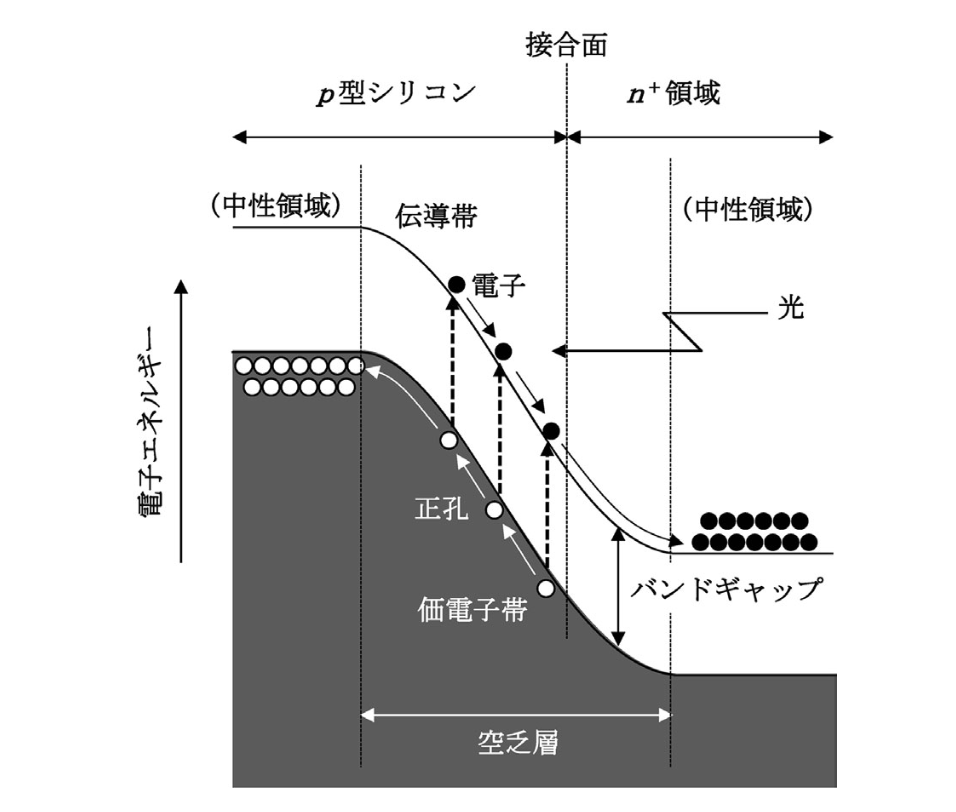
\includegraphics[scale=0.8]{./fig/photoconductive-effect.png}
	\caption{pn接合におけるエネルギーバンド\cite{sdfnvd}}
	\label{fig:photoconductive-effect}
\end{figure}

\subsection{追記:吸収端波長(absorption edge wavelength)\cite{11300202640}}
上述した,光導電効果を生じるには,フォトンエネルギーと半導体のエネルギーギャップ$E_{G}$の間で,\weq{FEG}を満たす必要がある.
\begin{equation}
	\varepsilon=h\frac{c}{\lambda}\geq E_{g}
	\label{eq:FEG}
\end{equation}
この式を変形して,波長$\lambda$について解くと\weq{lambda}を得る.
\begin{equation}
	\lambda \geq \frac{hc}{E_{G}}
	\label{eq:lambda}
\end{equation}
この式で等号の場合の$\lambda$を特に吸収端波長といい,$\lambda_{c}$で表す.
この波長より短い光は電子正孔対を生成できるため,フォトンのエネルギーはそれに消費されてしまう.
一方,$\lambda_{c}$より長い波長の光は,電子正孔対を生成できないため,吸収されないで半導体を通過する.

\subsection{追記:光起電力効果(photovoltaic effect)\cite{113002054832640}}
\label{photovoltaic-effect}
\wfig{pnl}に示すようなpn接合半導体に,吸収端波長より短い波長の光を照射する.
光強度は右奥の方にいくに従い,図(b)のように減少する.
ところで,pn接合間には,図(c)に示すようにもともと拡散電位差が生じている(n型の方が正に帯電).
したがって,光が入射することによって生じた電子正孔対は,光を照射した瞬間は図(c)のようであるが,その直後,空乏層中に発生した電子はドリフト現象により,拡散電位によって生じている伝導帯の坂を下り,左側のn側へ移動する.\\
空乏層より右側のp領域で発生した電子は,空乏層に近い領域の電子密度が低下したため,拡散現象により,空乏層側に移動していく.\\
その結果,n側の負の電荷量およびp側の正の電荷量が増加し,n側のエネルギーが相対的に高くなり,両者の電位差が減少する.
図(d)がこの状況を示す.この状態は,pn結合ダイオードに準バイアスとして$v_{D}$を加えたことに相当している.
つまり,$v_{D}$という起電力がp側を正,n側を負に発生することになる.
光強度を大きくしていくと,n側の電子のエネルギーがさらに高まり,ついに,エネルギーバンドがフラットになってしまい,これ以上の起電力は得られなくなる.
最後に,\wtab{tigai}に光導電効果と光起電力効果の違いについてまとめた表を示す.

\begin{figure}[h]
	\centering
	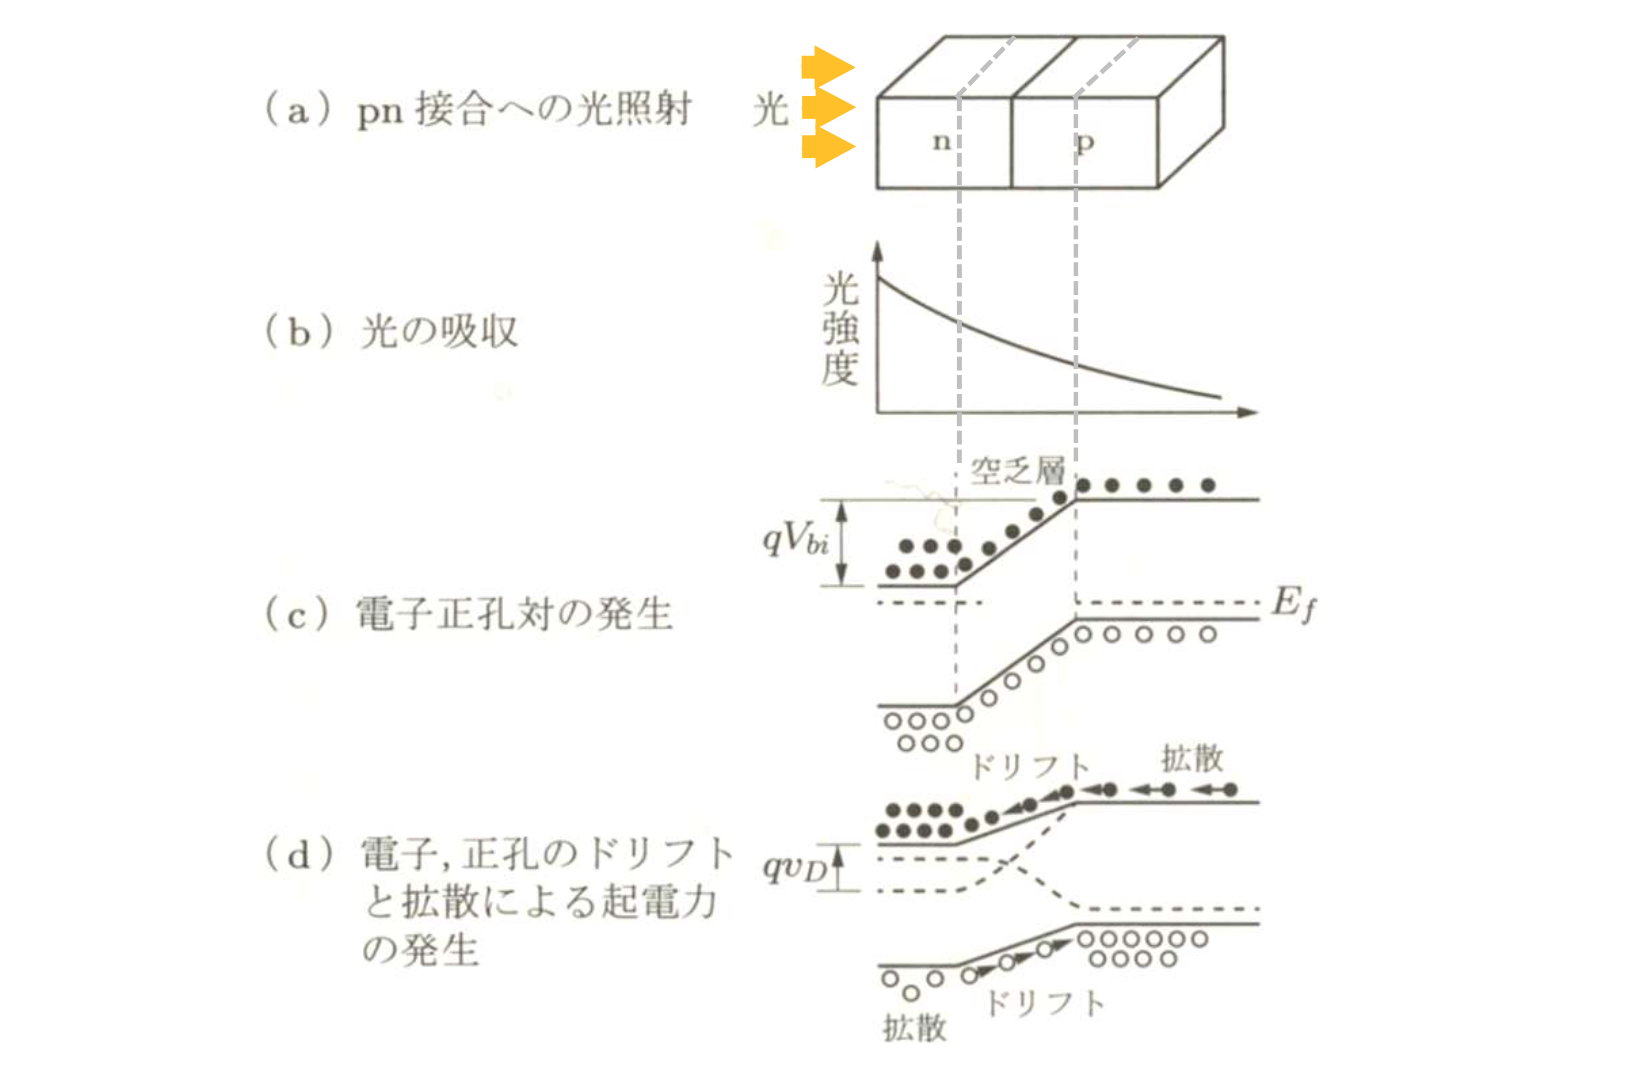
\includegraphics[scale=0.45]{./fig/pnl.png}
	\caption{光起電力効果の機構\cite{113002054832640}}
	\label{fig:pnl}
\end{figure}

\begin{table}[h]
\centering
\caption{光導電効果と光起電力効果の違い\cite{dfkljbn}}
\label{tab:tigai}
\begin{tabular}{ccc}
\hline
     & 光導電効果  & 光起電力効果 \\
     \hline
現象   & 
\begin{tabular}[c]{@{}c@{}}自由キャリアの増加\\ (導電率の増加)\end{tabular} & 起電力の発生 \\
内部電界 & なし       & あり     \\
外部電源 & 必要      & 不要     \\
利用例  & フォトセル(光検出器)       & 太陽電池  \\
\hline
\end{tabular}
\end{table}

\subsection{変更:太陽電池(solar cell)}
太陽電池は様々な種類のものがあるが,本実験では最も基本的な構造である結晶シリコン太陽電池(Crystalline silicon solar cell)を用いる.
結晶シリコン太陽電池の構造は,\wfig{fig3}のような上段がn 形半導体,下段がp 形半導体となっており,pn結合している.
\wfig{fig4}で示すように,光が照射されると,光起電力効果が発生する.(\ref{photovoltaic-effect})
この起電力は,光が照射されている間は持続し外部に負荷を接続しておけば電力を供給することができる.
また,電子は負荷を通ってp形半導体に戻り,正孔と結合する.
\begin{figure}[htb]
	\centering
	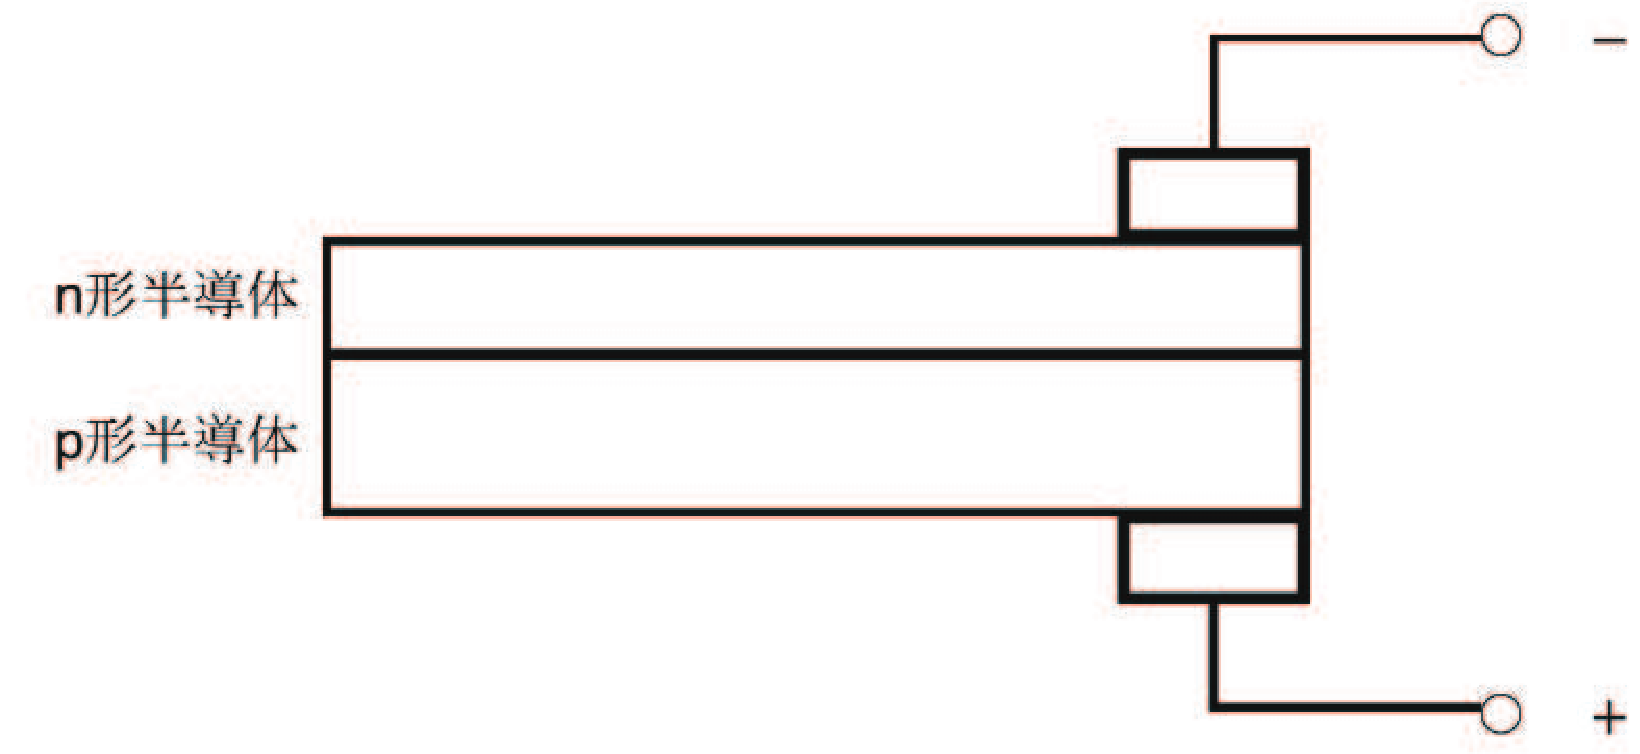
\includegraphics[width=6.3cm]{./fig/fig3.eps}
	\caption{結晶シリコン太陽電池の構造}
	\label{fig:fig3}
\end{figure}

\begin{figure}[htb]
	\centering
	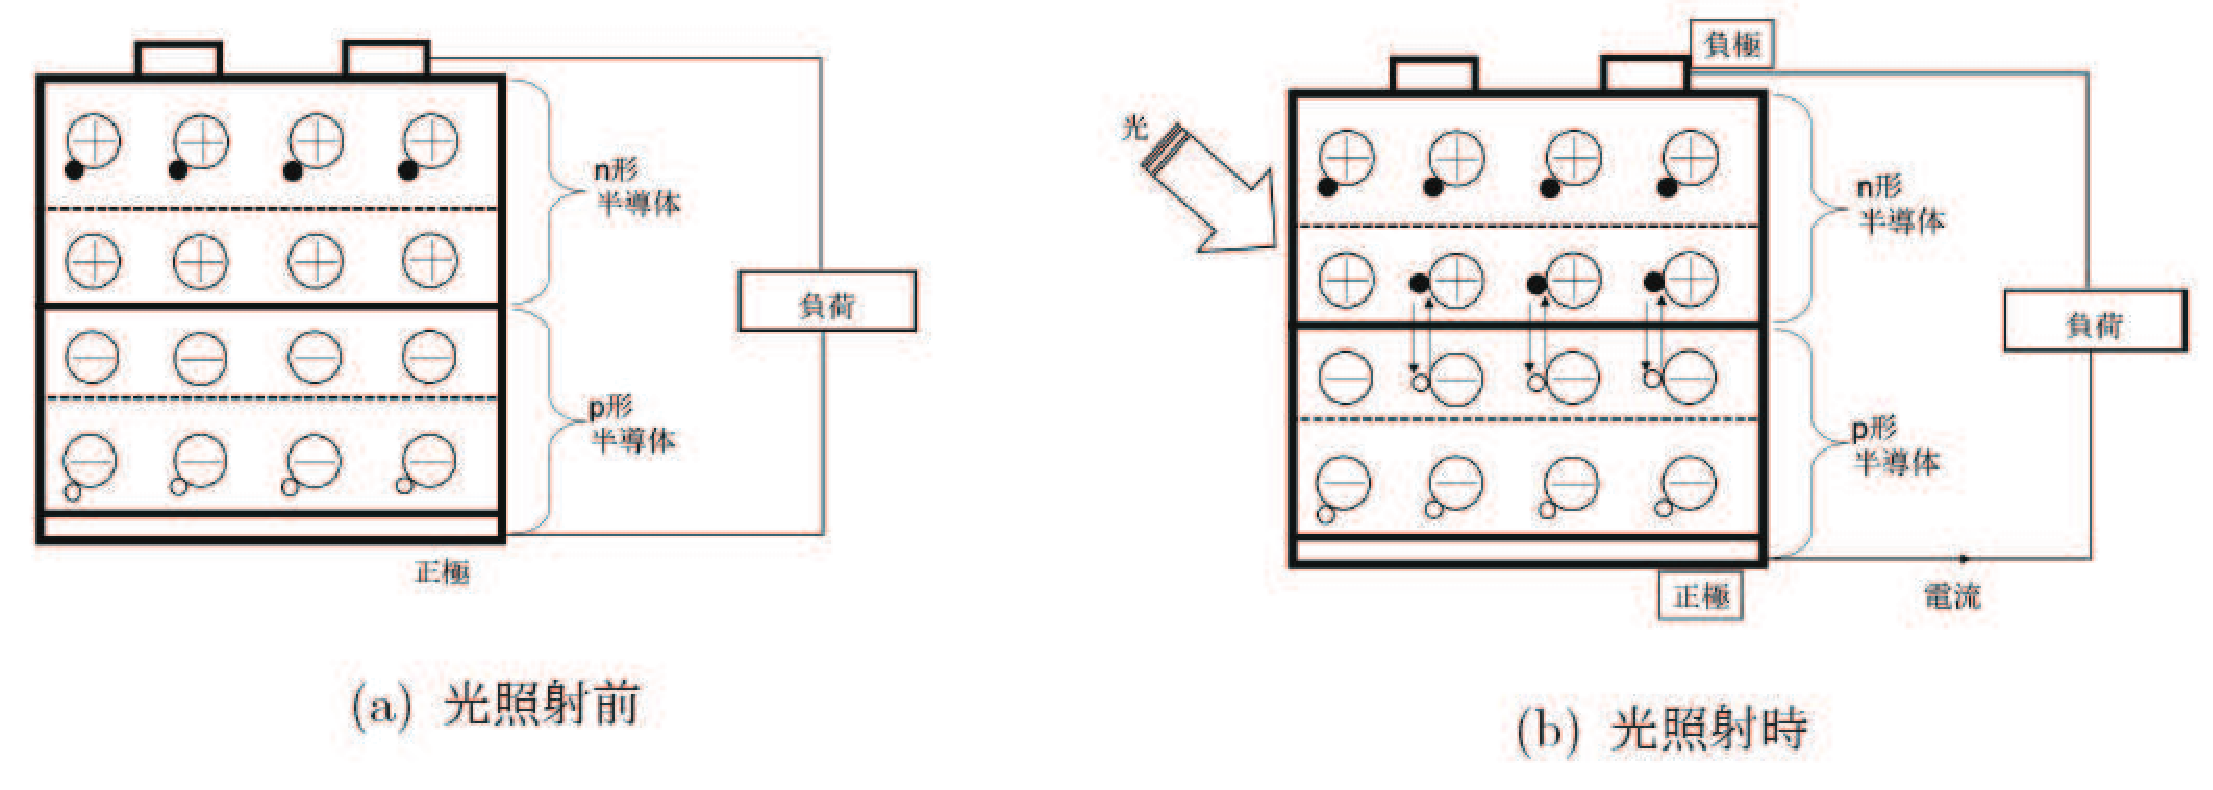
\includegraphics[width=12cm]{./fig/fig4.eps}
	\caption{太陽電池の動作原理}
	\label{fig:fig4}
\end{figure}

太陽電池の電流--電圧特性は\wfig{fig5}に示したようなダイオードの特性を下にシフトした特性となる.
ここで電流値は負の値になるが,正に消費と考えていたので負の値は発電していることを意味する.
一般的には,発電した電力も正の値で表現するので,縦軸を反転させる(\wfig{fig5}参照).
また,太陽電池の電流--電圧特性をI-Vカーブ,電力--電圧特性をP-Vカーブと呼ぶ.
\wfig{fig6}に示すように,I-V カーブは第1象限のみを表示する.

\subsection{追記:発電電力}
電圧が0\,\rm{V}になる(短絡する)時の電流を短絡電流($I_{\mathrm{sc}}$),電流が0\,\rm{A}になる電圧を解放電圧($V_{\mathrm{oc}}$)と呼ぶ.
また,縦軸を電力とした\wfig{fig6}に示すP-Vカーブより,太陽電池はどのようなどのような電圧で利用しても同じ電力を得られるわけではない.
太陽電池を有効に活用するためには,発電電力が最大になる最大電力点で利用する必要がある.

ここで,発電電力が最大になる電力を最大電力($P_{\mathrm{max}}$),その時の電圧を最適動作電圧($V_{\mathrm{pm}}$) と呼ぶ.
$P_{\mathrm{max}}$は,気象条件によって大きく変化し$V_{\mathrm{pm}}$も変化してしまう.
そのため,太陽電池を利用したシステム(太陽光発電システム)では,常に$P_{\mathrm{max}}$ を追従する制御であるMPPT制御(Maximum Power Point Tracking:最大電力点追尾)が具備されている.
MPPTには様々な手法があるが,その手法を考える上でも太陽電池のI-Vカーブの測定は非常に重要である.

\begin{figure}[htb]
	\centering
	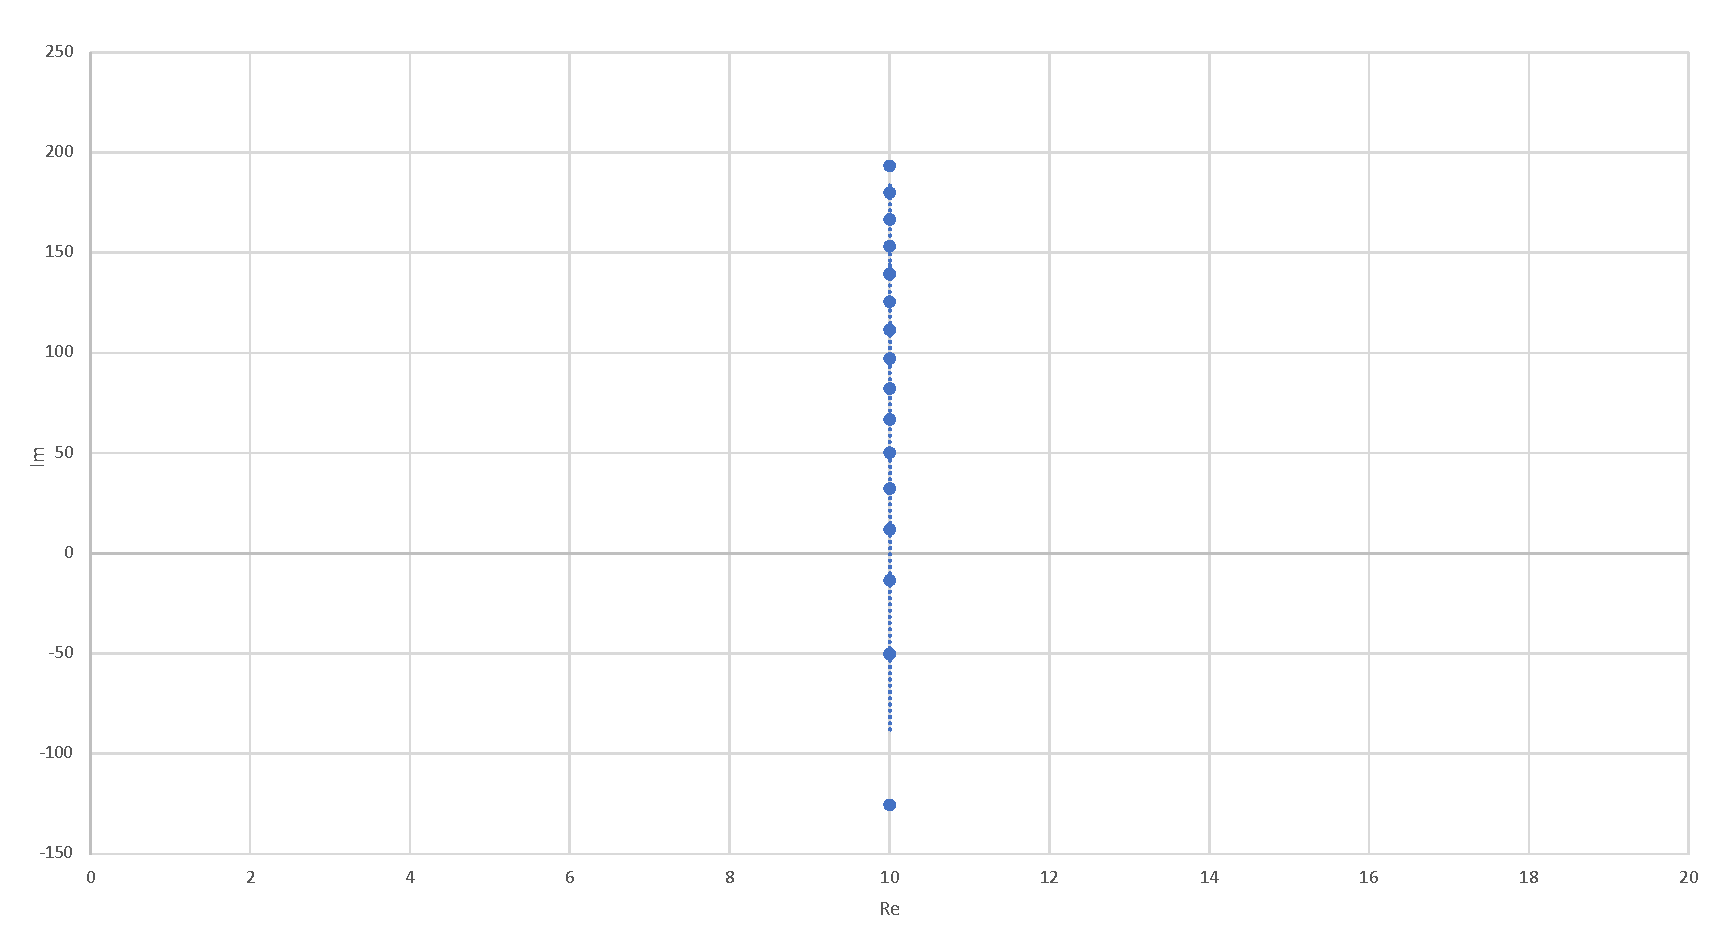
\includegraphics[width=8.5cm]{./fig/fig5.eps}
	\caption{ダイオードと太陽電池の電流--電圧特性}\
	\label{fig:fig5}
\end{figure}
\begin{figure}[htb]
	\centering
	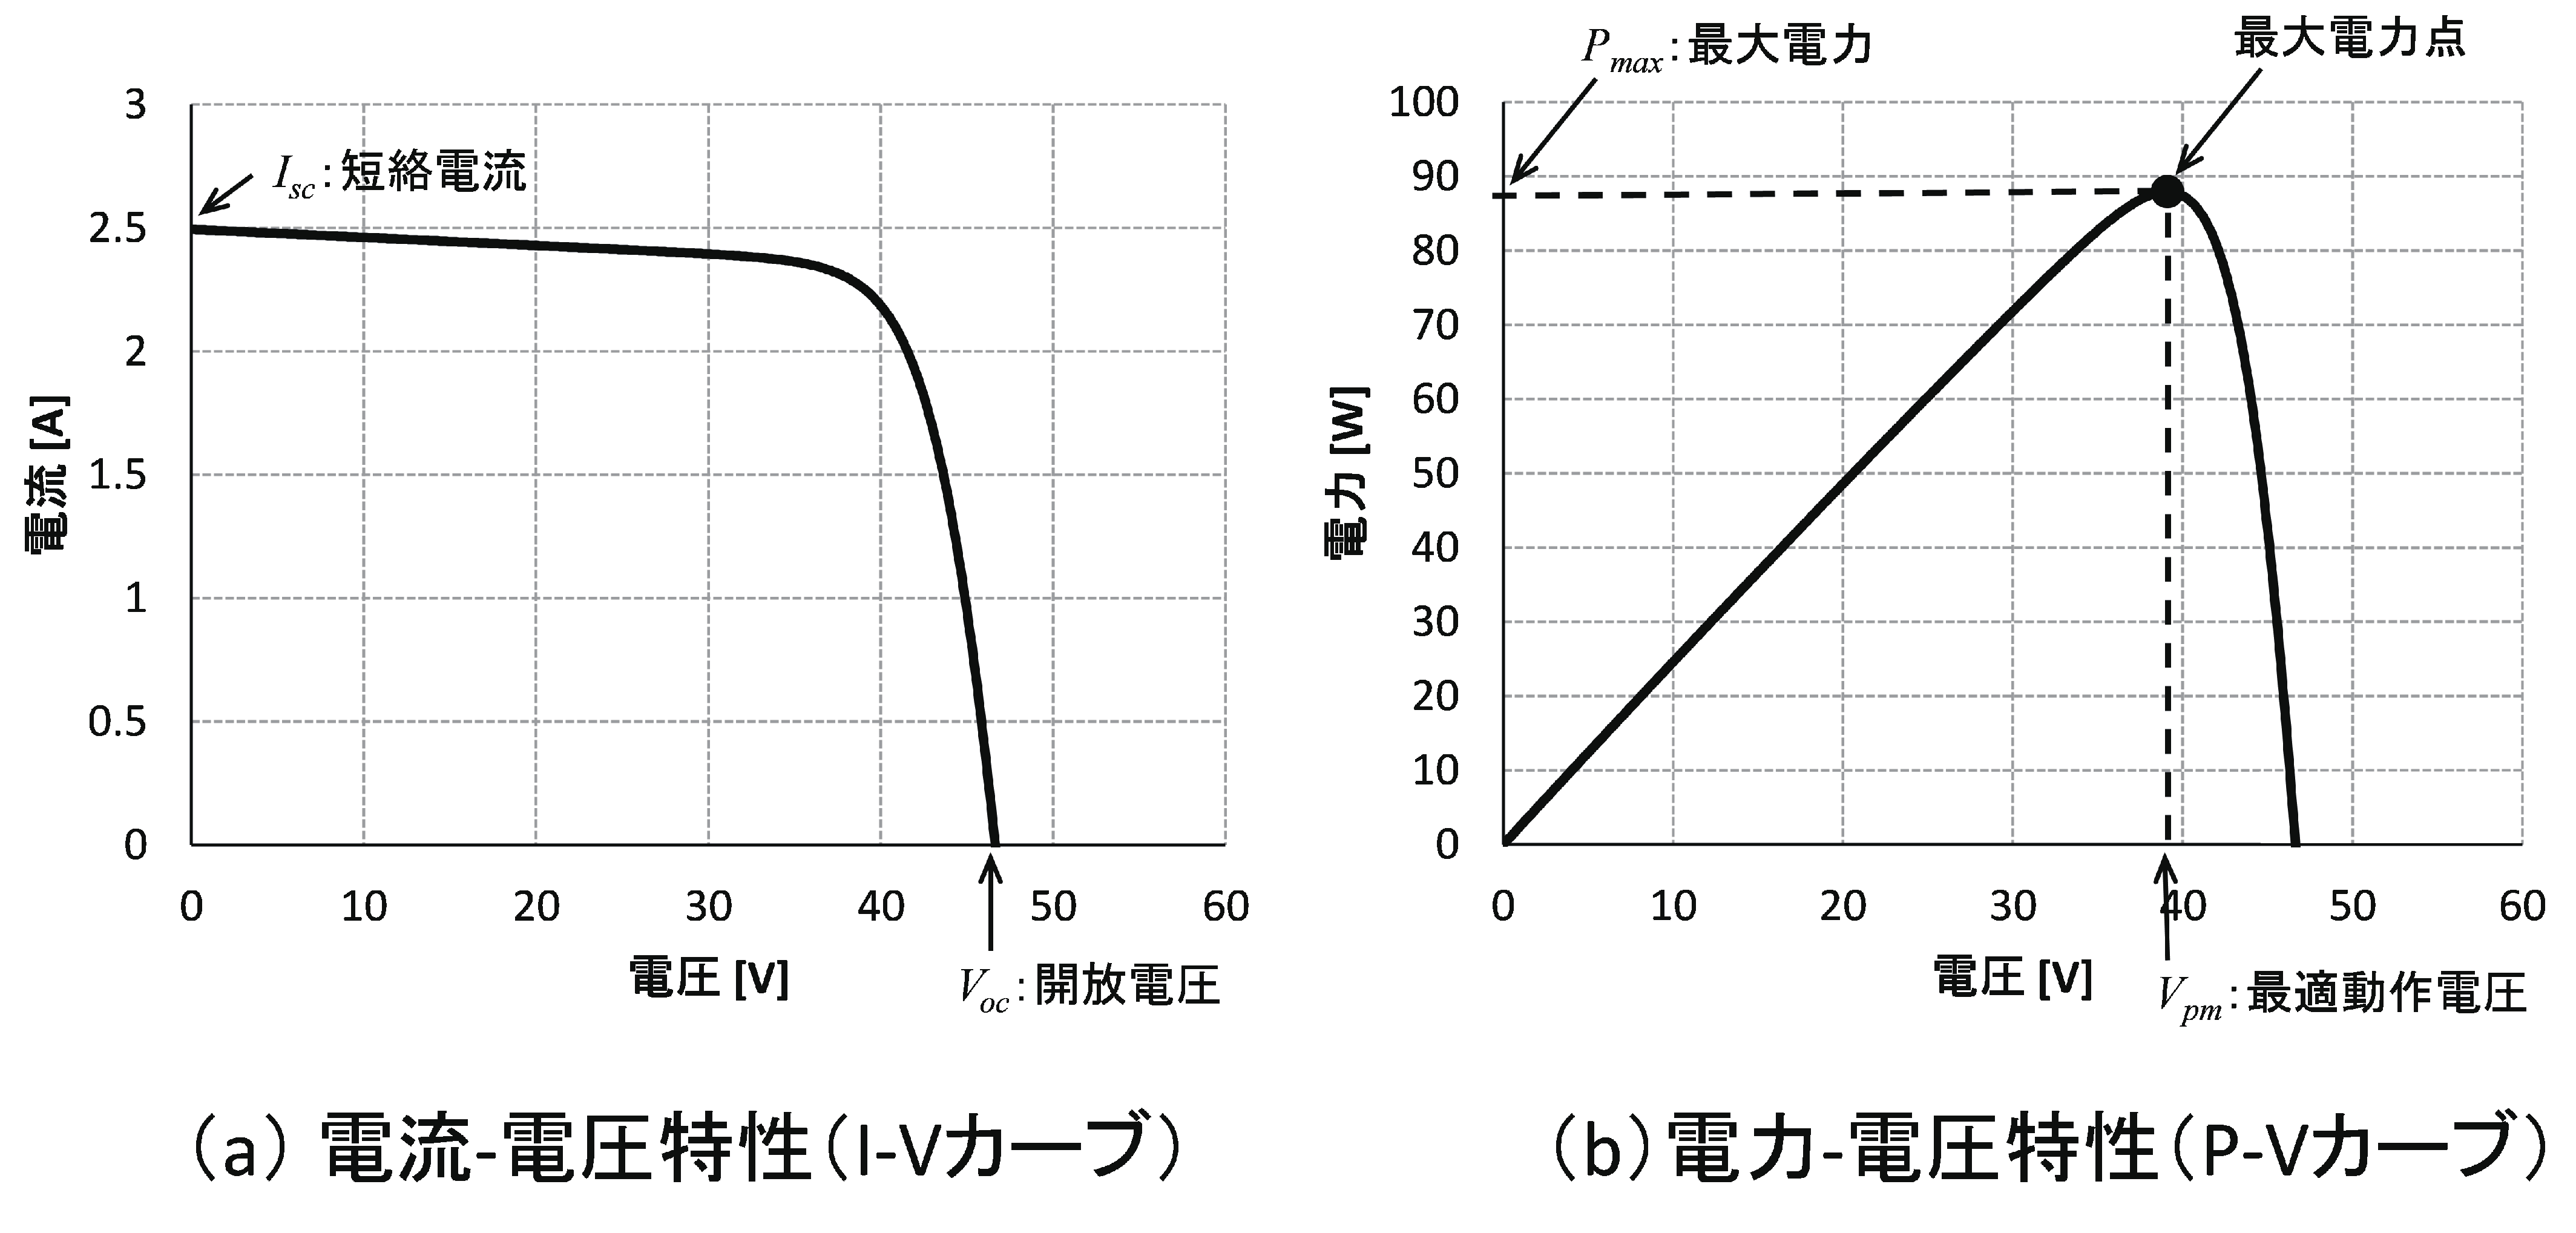
\includegraphics[width=10.3cm]{./fig/fig6.eps}
	\caption{太陽電池の発電特性(左:I--Vカーブ,右:P--Vカーブ)}
	\label{fig:fig6}
\end{figure}